\documentclass{beamer}
\usepackage[T1]{fontenc}
\usepackage[utf8]{inputenc}
\usepackage[ngerman]{babel} 
\usepackage{fancyvrb}
\usepackage{amsmath}
\usepackage{amssymb}
\usepackage{libertine}
\usepackage{courier}
\usepackage{hyperref}
\usepackage[style=authoryear,backend=biber]{biblatex}
\usepackage[babel]{csquotes}
\usepackage{booktabs}
\usepackage{multirow}
\addbibresource{literatur.bib}
\renewcommand*{\bibfont}{\footnotesize}

\makeatletter
\def\url@foostyle{%
  \@ifundefined{selectfont}{\def\UrlFont{\sf}}{\def\UrlFont{\footnotesize\ttfamily}}}
\makeatother
\urlstyle{sf}

\usepackage{tikz}
\usetikzlibrary{shapes,arrows,decorations.pathmorphing,backgrounds,positioning,fit,petri}
\tikzstyle{latent}=[circle,draw=black,semithick,inner sep=0pt,minimum size=10mm]
\tikzstyle{manifest}=[rectangle,draw=black,semithick,inner sep=0pt,minimum size=10mm]
\tikzstyle{const}=[regular polygon,regular polygon sides=3,draw=black!30,semithick,inner sep=0pt,minimum size=10mm]
\tikzstyle{resid}=[inner sep=0pt,minimum size=4mm]
\tikzstyle{corr}=[<->,shorten >=1pt,shorten <=1pt,>=stealth',semithick]
\tikzstyle{coef}=[->,shorten >=1pt,shorten <=1pt,>=stealth',semithick]
%\tikzset{venn circle/.style={draw,circle,minimum width=2cm,fill=#1,opacity=0.6}}
\tikzset{venn circle/.style={draw,circle,minimum width=2cm}}

%-------------------------------------------------------------------
\beamertemplatenavigationsymbolsempty
\makeatletter
\setbeamertemplate{footline}{
  \leavevmode%
  \hbox{%
  \begin{beamercolorbox}[wd=.333333\paperwidth,ht=.5cm,dp=1ex,left]
    {author in head/foot}%
    \hspace{.05cm}
    %
\includegraphics[height=0.15cm]{80x15.png}
    \hspace{.05cm}
    \usebeamerfont{author in head/foot}\insertauthor
  \end{beamercolorbox}%
  \begin{beamercolorbox}[wd=.666666\paperwidth,ht=.5cm,dp=1ex,right]
    {date in head/foot}%
    \vspace{-.1cm}
    %
\includegraphics[height=0.3cm]{150px-Uni_Mannheim_Siegel.png}
    \hspace{.05cm}
    %
\includegraphics[height=0.3cm]{sswml_logo2.png}
  \end{beamercolorbox}}%
  \vskip0pt%
}
\makeatother

%-------------------------------------------------------------------
\RecustomVerbatimEnvironment
  {Verbatim}{Verbatim}
  {frame=single,gobble=4,formatcom=\color{blue!50!black},}
%fontsize=\footnotesize
%-------------------------------------------------------------------
\title{Machine Learning} 
\subtitle{-- in 90 Minuten}
\author{Jonas Beste \& Arne Bethmann}
%\date{\footnotesize \url{https://gitlab.com/bethm/sem90}}

%-------------------------------------------------------------------
\begin{document}

%-------------------------------------------------------------------
\begin{frame}
  \titlepage
\end{frame}

%-------------------------------------------------------------------
\begin{frame}
  \frametitle{Überblick}
  \tableofcontents
\end{frame}

\section{Konzepte und Terminologie}
%-------------------------------------------------------------------
\begin{frame}
  \frametitle{Was ist Machine Learning}
  
  \begin{itemize}
  \item Machine Learning wird u.a. auch Statistical Learning genannt
  \item Darunter ist eine umfangreiches Auswahl an Verfahren zur Auswertung von Daten zu verstehen
  \item Diese umfassen weit mehr als den Ansatz der linearen Regression
  \item Algorithmen die von Daten lernen können
  \item Ermöglicht den Umgang mit großen Datenmengen
  \end{itemize}  
\end{frame}

%-------------------------------------------------------------------
\begin{frame}
  \frametitle{Grundlegendes}  
  \begin{itemize}
  \item Verwendung vorrangig für Vorhersagen (\emph{predictions}), aber auch für Schätzungen (\emph{estimations})
  \item Unterscheidung zwischen \emph{supervised} und \emph{unsupervised Learning} (Output beobachtet oder nicht)
  \item Unterscheidung zwischen Regressions- und Klassifikationsproblemen (quantitative und qualitative Variablen)
  \item Trainings- und Testdaten:
      \begin{itemize} 
   \item Lernen des Klassifikators (Konstruktion des Modells) anhand von Trainingsdaten
  \item Interesse an guter Vorhersage bislang unbekannter Fälle (Testdaten)
 \end{itemize}  
 \end{itemize}  
 \end{frame}

\section{Modellauswahl}

%-------------------------------------------------------------------
\begin{frame}
  \frametitle{Genauigkeit und Interpretierbarkeit}  
  \begin{itemize}
  \item Abwägung zwischen Genauigkeit und Interpretierbarkeit von Methoden
  \item Manche Methoden sind flexibles (weniger restriktiv) als andere
  \item Flexible Methoden können sich sehr gut den Daten anpassen und ermöglichen so sehr genaue Vorhersagen
  \item Restriktive Methoden hingegen sind meist deutlich besser zu interpretieren (bevorzugt bei Inferenz)
  \item Problem des \emph{Overfitting}: Zu starke Anpassung an die Trainingsdaten, wodurch Testdaten ungenügend vorhergesagt werden
  \item Daher führen weniger flexible Methoden häufig zu besseren Ergebnissen
  \end{itemize}  
\end{frame}

%-------------------------------------------------------------------
\begin{frame}
  \frametitle{Bewertung von Statistical Learning Methoden} 
  \begin{itemize}
  \item Keine Methode ist die allgemein Beste für alle Fragen und Daten
  \item Daher kommt der Auswahl der geeigneten Methode eine besondere Bedeutung zu
  \item Maß für die Qualität: Wie gut passen die Vorhersagen tatsächlich zu den beobachteten Daten?
  \item Bei regressionsbasierten Vorhersagen wird meistens der \emph{mean squared error} (MSE) herangezogen: \newline
\begin{center}
      $\frac{1}{n} \sum\limits_{i=1}^{n}(y_{i}-\hat{f}(x_{i}))^2$
  \end{center}  \item Bei Klassifikationen ergibt sich die Fehlerrate aus dem Anteil falsch zugeordneter Fälle:
  \newline
\begin{center}
      $\frac{1}{n} \sum\limits_{i=1}^{n}I(y_{i}\neq\hat{y_{i}})$
  \end{center}  
  \end{itemize}  
\end{frame}

%-------------------------------------------------------------------
\begin{frame}
  \frametitle{Bias-Variance Trade-Off}  
  \begin{itemize}
  \item Bei Erhöhung der Flexibilität sinkt die Verzerrung und steigt die Varianz
  \item Auswahl einer Methode die geringe Verzerrung und geringe Varianz aufweist
  \item Abwägung zwischen Ausmaß an Verzerrung und Varianz notwendig
  \end{itemize}  
\end{frame}

%-------------------------------------------------------------------
\begin{frame}
  \frametitle{Resampling Methoden} 
  \begin{itemize}
  \item Resampling Methoden können verwendet werden um Aussagen über die Eignung von Modellen zu machen
  \item Technik um zu prüfen, wie sich die Modelle bei unabhängigen Daten verhalten (Overfitting)
  \item Zu dem Resampling Methoden gehört die Kreuzvalidierung sowie das Bootstrapping
  \item Kreuzvalidierung kann verwendet werden um die Performance eines Modells zu bewerten (\emph{model assessment}) oder den geeigneten Grad an Flexibilität zu bestimmen (\emph{model selection})
    \end{itemize}  
\end{frame}

\begin{frame}
  \frametitle{Kreuzvalidierung} 
  \begin{itemize}
   \item Validation Set Approach: 
   \begin{itemize}
  \item Unterteilt die Beobachtungen zufällig in einen Trainingsset und einen Validierungsset
  \item Das Modell wird am Trainingsset konfiguriert und am Validierungsset getestet
  \end{itemize}    
  \item k-Fold Cross-Validation: 
     \begin{itemize}
  \item Unterteilt die Beobachtungen zufällig in k ungefähr gleich große Teilmengen
  \item Verwendet k-1 Teilmengen zur Erstellung des Modells und die verbleibende Teilmenge zur Validierung
  \item Berechnet k Modelle, wobei jede Teilmenge genau einmal als Validierungsset dient
  \item Die Ergebnisse der einzelnen Modelle können dann kombiniert werden
  \item Jede Beobachtung wird für Training und genau einmal für die Validierung verwendet
  \item In der Regel wird k = 5 oder k = 10 gewählt
  \end{itemize}  
  \end{itemize}  
\end{frame}

\section{Naive Bayes}

%%-------------------------------------------------------------------
\begin{frame}
  \frametitle{Naive Bayes}  
  \begin{itemize}
  \item Simpler probabilistischer Klassifikator basierend auf der Anwendung des Bayes Theorem
  \item Starke (naive) Annahme der Unabhängigkeit zwischen den erklärenden Merkmalen
  \item Dabei wird jede Beobachtung der Klasse zugeteilt, die bei gegebenen Prediktoren am wahrscheinlichsten ist
  \item So gesehen ist naive Bayes ein Modell bedingter Wahrscheinlichkeit und kann dargestellt werden als:
  \newline
   \begin{center}
   $p(C_{k}|x) = \frac{p(C_{k}) \times p(x|C_{k})}{p(x)}$
   \end{center}
  \end{itemize}  
\end{frame}

%-------------------------------------------------------------------
\begin{frame}
  \frametitle{Naive Bayes -- Beispiel}  
  \begin{itemize}
  \item Zeuge hat eine Person gesehen, konnte aber das Geschlecht der Person nicht erkennen
  \item Bekannt sind nur Informationen zu Größe und Farbe der Klamotten
  \item Die Person war kleiner als 170 cm und trug helle Klamotten
  \item Handelt es sich dabei um eine Frau oder um einen Mann?
  \item Um die Frage zu beantworten, kann auch eine Reihe von Beobachtungen zurückgegriffen werden
  \end{itemize}  
\end{frame}

%-------------------------------------------------------------------
\begin{frame}
  \frametitle{Naive Bayes -- Example}  
  Beobachtungen \\
  \vspace{.5em}
  {\footnotesize
  \begin{tabular}{rrrr}
  \midrule
  Fall & Geschlecht & über 170 cm & dunkle Klamotten \\
\midrule  
  1  & Frau & nein & ja \\
  \addlinespace
  2  & Frau & nein & nein \\
  \addlinespace
  3  & Mann & ja & ja \\
    \addlinespace
  4  & Frau & ja & nein \\
    \addlinespace
  5  & Mann & nein & nein \\
    \addlinespace
  6  & Mann & ja & ja \\
  \midrule
  \end{tabular}
  } 
\end{frame}

%-------------------------------------------------------------------
\begin{frame}
  \frametitle{Naive Bayes -- Beispiel}  
  \begin{itemize}
  \item Bestimmung der bedingten Wahrscheinlichkeit:
\vspace{.4cm}  
\newline 
\vspace{.4cm}
  $p(\text{Frau}|\text{<170cm, hell}) = \frac{p(\text{<170cm}|\text{Frau}) \times p(\text{hell}|\text{Frau}) \times p(Frau)}{p(<170cm) \times p(hell)}$
 \newline 
 \vspace{.4cm}
  $p(\text{Mann}|\text{<170cm, hell}) = \frac{p(\text{<170cm}|\text{Mann}) \times p(\text{hell}|\text{Mann}) \times p(Mann)}{p(<170cm) \times p(hell)}$
\newline 
\vspace{.4cm}
    $p(\text{Frau}|\text{<170cm, hell}) > p(\text{Mann}|\text{<170cm, hell})$
  \item Die Person wird als Frau klassifiziert
  \end{itemize}  
\end{frame}

\section{k-nearest-neighbor}

%-------------------------------------------------------------------
\begin{frame}
  \frametitle{k-nearest-neighbor}  
  \begin{itemize}
  \item Eine einfache Methode die bei vielen Problem sehr gut funktioniert
  \item Ein Objekt wird der Klasse zugeteilt, die bei einer bestimmten Anzahl k der nächsten Nachbarn im Merkmalsraum am häufigsten vorkommt
  \item k ist dabei eine natürliche in der Regel niedrige Zahl
  \item Die bedingte Wahrscheinlichkeit des Objektes $x_{0}$ für die Klasse $j$ ist der Anteil der Nachbar $N_{0}$ die dieser Klasse angehören:
  \newline
\begin{center}
    $Pr(Y=j|X=x_{0}) = \frac{1}{K}\sum\limits_{i \in N_{0}}I(y_{i}=j) $
  \end{center}  
  \item Ein Schwachpunkt dieses Algorithmus ist seine Sensibilität auf lokale Strukturen in den Daten (Overfitting)
  \end{itemize}  
\end{frame}

%-------------------------------------------------------------------
\begin{frame}
  \frametitle{k-nearest-neighbor -- Beispiel}  
 %\centering
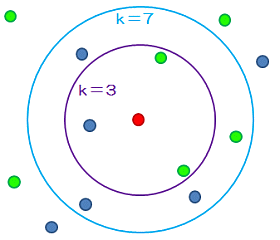
\includegraphics[scale=.4]{knn.png} \\
%\vspace{2em}
\flushleft
\emph{\tiny Quelle: \url{http://www.nag-j.co.jp/nagdmc/img/knn.gif}}
\normalsize
 \begin{itemize}
  \item Roter Punkt ist zu klassifizieren
  \item k = 3: Rot wird grün klassifiziert 
  \item k = 7: Rot wird blau klassifiziert 
  \item Die Distanz zu den Nachbarn kann als Gewichtung mit aufgenommen werden
  \end{itemize}  
\end{frame}

\section{Entscheidungsbäume}

%-------------------------------------------------------------------
\begin{frame}
  \frametitle{Entscheidungsbäume}  
  \begin{itemize}
  \item Caret: Classification and regression tree
  \item Abfolge von binären Entscheidungen, die als Baum mit Blätter, Zweige und Knoten darstellbar sind
  \item Top-down Induktion: Beginnt an der Wurzel (Startknoten) des Baumes und verzweigt sich mit jedem Schritt
  \item Die Entscheidungen werden so getroffen, dass die Knoten hinsichtlich der Zielvariable möglichst homogene Klasse darstellen
  \item In den Blättern (Endknoten) wird eine Zuordnung zu der Klasse getroffen, die dort am häufigsten vorkommt (oder Mittelwert bei Regressionsbäumen)
   \item \emph{Pruning} eines großen Entscheidungsbaums, um Overfitting zu vermeiden
   \item Entscheidungsbäume sind gut interpretierbar, aber nicht sehr akkurat
 \end{itemize}  
\end{frame}

%-------------------------------------------------------------------
\begin{frame}
  \frametitle{Entscheidungsbäume -- Beispiel}  
  \begin{center}
%  \vspace{.5em}
  \scalebox{.9}{
  \begin{tikzpicture}   

    % Knoten
    \node[manifest] (ind1){\footnotesize Erwerb} (7,-7);
    \node[latent, label=below:{\footnotesize 0,04}] (dep1) [below left=1 and 1 of ind1] {\footnotesize N. arm};
    \node[latent, label=below:{\footnotesize 0,30}] (dep2) [below right=1 and 1 of ind1] {\footnotesize N. arm}; 
    
    % Entscheidungen
    \draw [coef] (ind1) to node[auto] {\footnotesize ja} (dep1); 
    \draw [coef] (ind1) to node[auto] {\footnotesize nein} (dep2); 
 
  \end{tikzpicture}
  }
  \end{center}
\end{frame}

%-------------------------------------------------------------------
\begin{frame}
  \frametitle{Entscheidungsbäume -- Beispiel}  
  \begin{center}
%  \vspace{.5em}
  \scalebox{.9}{
  \begin{tikzpicture}   

    % Knoten
    \node[manifest] (ind1) {\footnotesize Erwerb} (7,-7);
    \node[latent, label=below:{\footnotesize 0,04}] (dep1) [below left=1 and 1 of ind1] {\footnotesize N. arm};
    \node[manifest, label={}] (dep2) [below right=1 and 1 of ind1] {\footnotesize Partner};
    \node[latent, label=below:{\footnotesize 0,22}] (dep3) [below left=1 and 1 of dep2] {\footnotesize N. arm};
    \node[latent, label=below:{\footnotesize 0,38}] (dep4) [below right=1 and 1 of dep2] {\footnotesize N. arm};
        
    % Entscheidungen
    \draw [coef] (ind1) to node[auto] {\footnotesize ja} (dep1); 
    \draw [coef] (ind1) to node[auto] {\footnotesize nein} (dep2); 
    \draw [coef] (dep2) to node[auto] {\footnotesize ja} (dep3); 
    \draw [coef] (dep2) to node[auto] {\footnotesize nein} (dep4);  
     
  \end{tikzpicture}
  }
  \end{center}
\end{frame}

%-------------------------------------------------------------------
\begin{frame}
  \frametitle{Entscheidungsbäume -- Beispiel}  
  \begin{center}
%  \vspace{.5em}
  \scalebox{.9}{
  \begin{tikzpicture}   

    % Knoten
    \node[manifest] (ind1) {\footnotesize Erwerb} (7,-7);
    \node[latent, label=below:{\footnotesize 0,04}] (dep1) [below left=1 and 1 of ind1] {\footnotesize N. arm};
    \node[manifest, label={}] (dep2) [below right=1 and 1 of ind1] {\footnotesize Partner};
    \node[latent, label=below:{\footnotesize 0,22}] (dep3) [below left=1 and 1 of dep2] {\footnotesize N. arm};
    \node[manifest, label={}] (dep4) [below right=1 and 1 of dep2] {\footnotesize Kinder};
    \node[latent, label=below:{\footnotesize 0,26}] (dep5) [below left=1 and .5 of dep4] {\footnotesize N. arm};
    \node[latent, label=below:{\footnotesize 0,60}] (dep6) [below right=1 and .5 of dep4] {\footnotesize arm};

    % Entscheidungen
    \draw [coef] (ind1) to node[auto] {\footnotesize ja} (dep1); 
    \draw [coef] (ind1) to node[auto] {\footnotesize nein} (dep2); 
    \draw [coef] (dep2) to node[auto] {\footnotesize ja} (dep3); 
    \draw [coef] (dep2) to node[auto] {\footnotesize nein} (dep4);  
    \draw [coef] (dep4) to node[auto] {\footnotesize ja} (dep5); 
    \draw [coef] (dep4) to node[auto] {\footnotesize nein} (dep6);  

  \end{tikzpicture}
  }
  \end{center}
\end{frame}

%-------------------------------------------------------------------
\begin{frame}
  \frametitle{Entscheidungsbäume -- Beispiel}  
  \begin{center}
%  \vspace{.5em}
  \scalebox{.9}{
  \begin{tikzpicture}   

    % Knoten
    \node[manifest] (ind1) {\footnotesize Erwerb} (7,-7);
    \node[latent, label=below:{\footnotesize 0,04}] (dep1) [below left=1 and 1 of ind1] {\footnotesize N. arm};
    \node[manifest, label={}] (dep2) [below right=1 and 1 of ind1] {\footnotesize Partner};
    \node[manifest, label={}] (dep3) [below left=1 and 1 of dep2] {\footnotesize P. Erw};
    \node[manifest, label={}] (dep4) [below right=1 and 1 of dep2] {\footnotesize Kinder};
    \node[latent, label=below:{\footnotesize 0,26}] (dep5) [below left=1 and .5 of dep4] {\footnotesize N. arm};
    \node[latent, label=below:{\footnotesize 0,60}] (dep6) [below right=1 and .5 of dep4] {\footnotesize arm};
    \node[latent, label=below:{\footnotesize 0,06}] (dep7) [below left=1 and .5 of dep3] {\footnotesize N. arm};
    \node[latent, label=below:{\footnotesize 0,52}] (dep8) [below right=1 and .5 of dep3] {\footnotesize arm};
    
    % Entscheidungen
    \draw [coef] (ind1) to node[auto] {\footnotesize ja} (dep1); 
    \draw [coef] (ind1) to node[auto] {\footnotesize nein} (dep2); 
    \draw [coef] (dep2) to node[auto] {\footnotesize ja} (dep3); 
    \draw [coef] (dep2) to node[auto] {\footnotesize nein} (dep4);  
    \draw [coef] (dep4) to node[auto] {\footnotesize ja} (dep5); 
    \draw [coef] (dep4) to node[auto] {\footnotesize nein} (dep6);  
    \draw [coef] (dep3) to node[auto] {\footnotesize ja} (dep7); 
    \draw [coef] (dep3) to node[auto] {\footnotesize nein} (dep8);  
    
  \end{tikzpicture}
  }
  \end{center}
\end{frame}

\section{Ensemble Learning}

%-------------------------------------------------------------------
\begin{frame}
  \frametitle{Bagging}  
  \begin{itemize}
  \item Bootstrap aggregation (Bagging) ist ein Verfahren um die Varianz von statistischen Modellen zu verringern und so aussagekräftigere Vorhersagemodelle zu erhöhen
  \item Hintergrund: Reduktion der Varianz durch Mittelwertbildung über mehrere Beobachtungen
  \item Ziehung von $B$ Trainingsdatensets aus dem ursprünglichen Trainingsdatenset (bootstrap)
  \item Bildung separater Modelle $\hat{f}^\ast_{b}(x)$ mit den einzelnen Trainingssets
  \item Mittelwertbildung der resultierenden Vorhersagen:
  \newline
\begin{center}
      $\hat{f}_{bag}(x)=\frac{1}{B}\sum\limits_{b=1}^{B}(\hat{f}^\ast_{b}(x))$
  \end{center}  
  \item Besonders effizient bei Verfahren mit hoher Varianz und geringem Bias (wie z.B. Entscheidungsbäumen)
  \end{itemize}  
\end{frame}

%-------------------------------------------------------------------
\begin{frame}
  \frametitle{Random Forest}  
  \begin{itemize}
  \item Ähnliches Verfahren wie Bagging für Entscheidungsbäume, nur dass bei jedem einzelnen Baum nur eine zufällige Auswahl der erklärenden Variablen berücksichtigt wird
  \item In der Regel wird Wurzel aller Predictoren
  \item Verringert die Korrelation der Vorhersagen zwischen den einzelnen Bäumen
  \item Hohe Korrelation führt zu geringerer Effizienz der Aggregation 
  \end{itemize}  
\end{frame}

%-------------------------------------------------------------------
\begin{frame}
  \frametitle{Boosting}  
  \begin{itemize}
  \item Weiteres Verfahren um die aussagekräftigere von Vorhersagemodellen zu erhöhen
  \item Kombination einzelnen für sich genommen schwachen Klassifikatoren
  \item Reduktion von Bias und Varianz
  \item Während beim Bagging die einzelnen Modelle unabhängig voneinander geschätzt werden, bauen diese beim Boosting aufeinander auf
  \item Erfolgt über Gewichtung der Daten
  \item Sehr effizient für Entscheidungsbäume
  \end{itemize}  
\end{frame}

\section{Weiteres}

%-------------------------------------------------------------------
\begin{frame}
  \frametitle{Weitere Techniken}  
  \begin{itemize}
  \item Weitere Klassifikationsmethoden (Logit, Probit und Diskriminanzanalyse)
  \item Modellauswahl (Ridge Regression und Lasso)
  \item Nichtlineare Modelle (Splines und additive Modelle)
  \item Support Vector Machines
  \item Neuronale Netze
  \item Unsupervised Learning (Hauptkomponentenanalyse und Clustern)
  \item ROC-Kurven, Sensitivität und Spezifität
  \item Weitere Ensemble Learning Techniken (Stacking)
  \end{itemize}  
\end{frame}


%-------------------------------------------------------------------
\end{document}
